\documentclass{IEEEtran}
\usepackage{graphicx, float}
\usepackage{soul}

\usepackage[hidelinks]{hyperref}
\usepackage[backend=biber]{biblatex}
\addbibresource{references.bib}

\newcommand{\makeNAMEFig}{%
\begin{figure}[tbp]
    \centering
    \includegraphics[width=\linewidth]{figures/NAME}
    \caption{CAPTION}
    \label{fig:NAME}
\end{figure}
}

\newcommand{\makeSampleSegFig}{%
\begin{figure}[tbp]
    \centering
    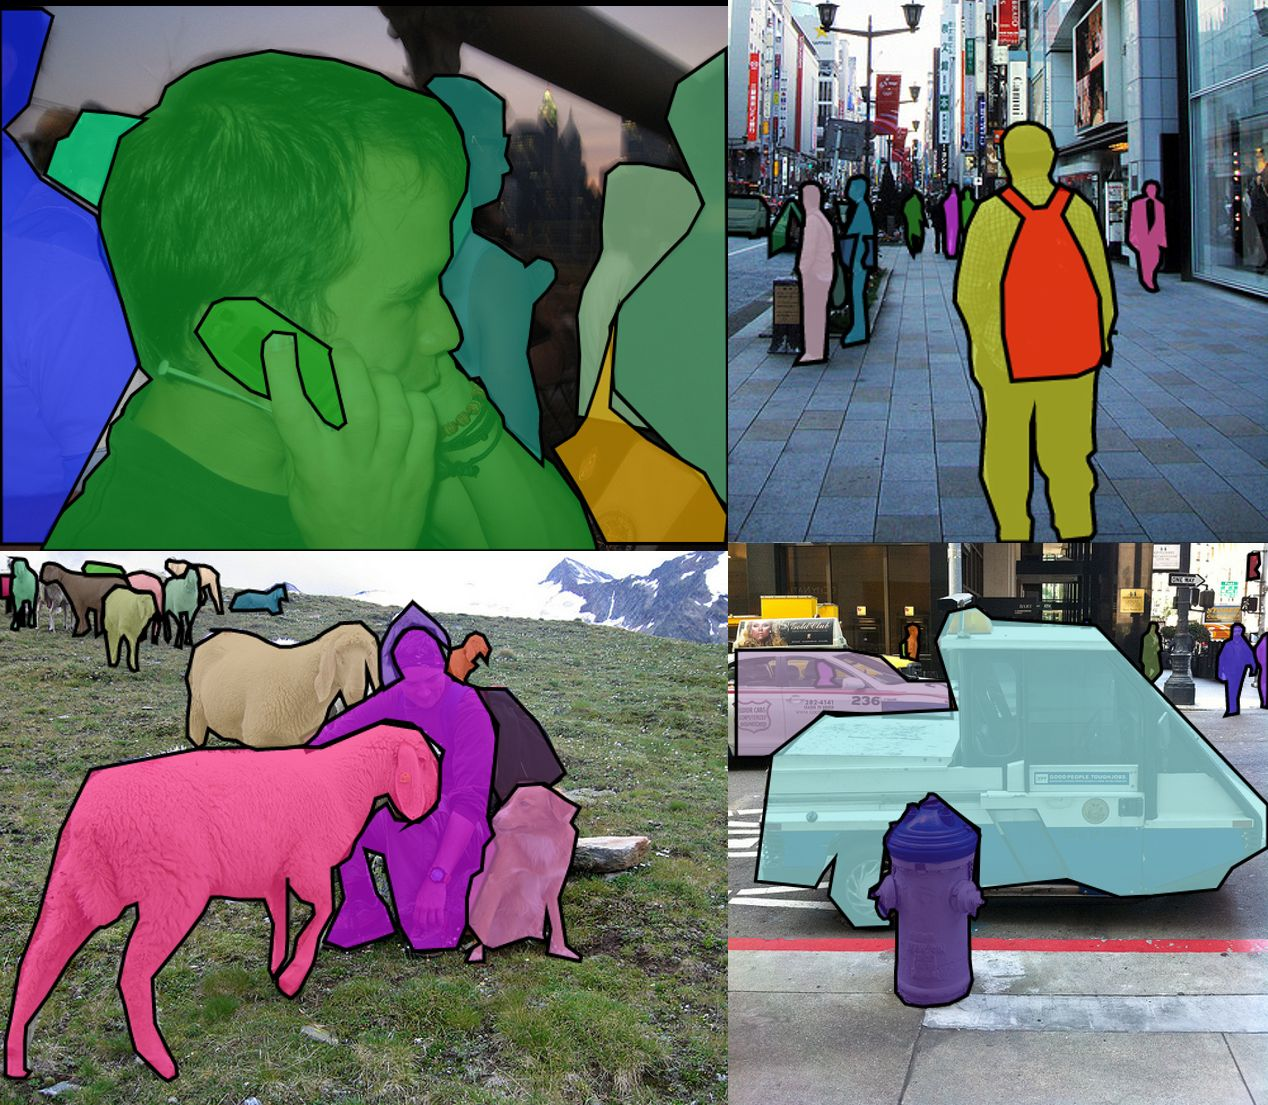
\includegraphics[width=0.75\linewidth]{figures/sampleSegData}
    \caption{Common use cases for semantic segmentation involve relatively few foreground objects, low-resolution data, and limited complexity per object. Images retrieved from \url{https://cocodataset.org/\#explore}.}
    \label{fig:sampleSegData}
\end{figure}
}

\newcommand{\makePcbFig}{%
\begin{figure}[tbp]
    \centering
    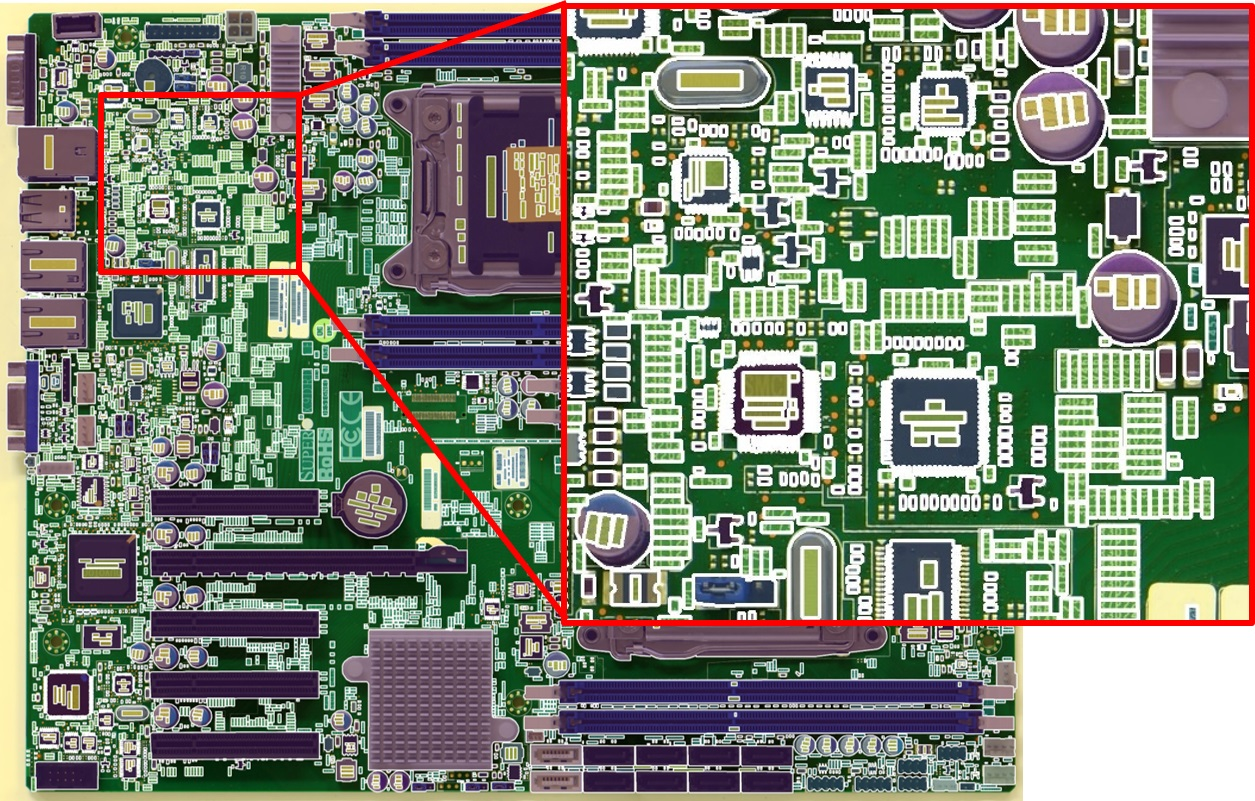
\includegraphics[width=\linewidth]{figures/pcb}
    \caption{Example PCB segmentation. In contrast to typical semgentation tasks, the scene contains over 4,000 objects with numerous complex shapes.}
    \label{fig:pcb}
\end{figure}
}


\newcommand{\makeFeedbackLoopFig}{%
\begin{figure}[tbp]
	\centering
	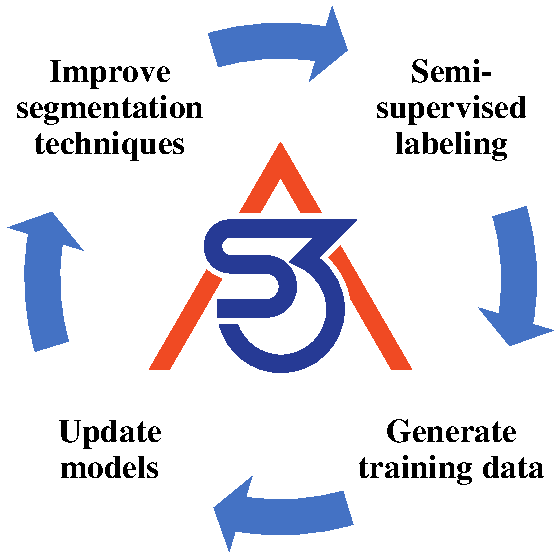
\includegraphics[width=0.5\linewidth]{figures/feedbackLoop}
	\caption{S3A's can iteratively annotate, evaluate, and update its internals in real-time.}
	\label{fig:feedbackLoop}
\end{figure}
}

\newcommand{\makeAppOverviewFig}{%
\begin{figure}[btp]
    \centering
    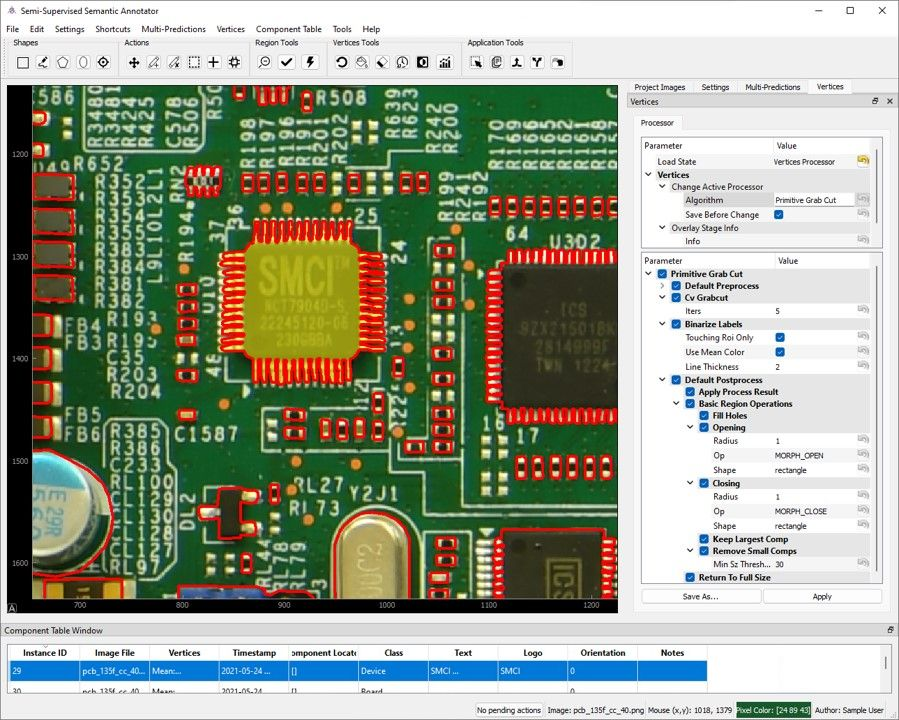
\includegraphics[width=\linewidth]{figures/appOverview}
    \caption{S3A's interface. The main view consists of an image to annotate, a component table of prior annotations, and a toolbar which changes functionality depending on context.}
    \label{fig:appOverview}
\end{figure}
}

\newcommand{\makeCropExportsFig}{%
\begin{figure}[tbp]
    \centering
    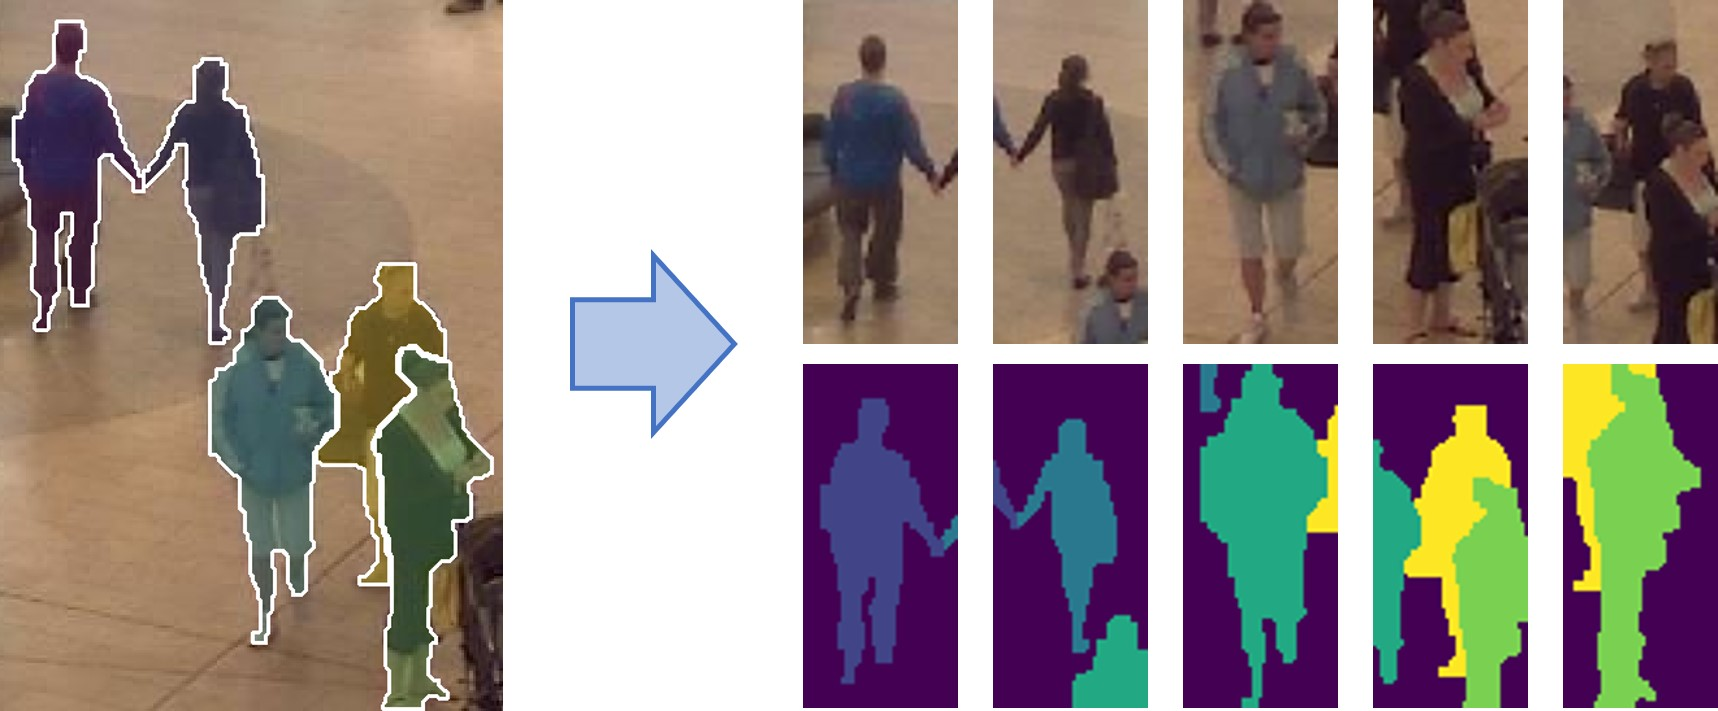
\includegraphics[width=\linewidth]{figures/cropExports}
    \caption{Multiple export formats exist, among which is a utility that crops components out of the image, optionally padding with scene pixels and resizing to ensure all shapes are equal. Each sub-image and mask is saved accordingly, which is useful for training on multiple forms of machine learning models.}
    \label{fig:cropExports}
\end{figure}
}

\newcommand{\makeRegionAnalyticsFig}{%
\begin{figure*}[tbp]
    \centering
    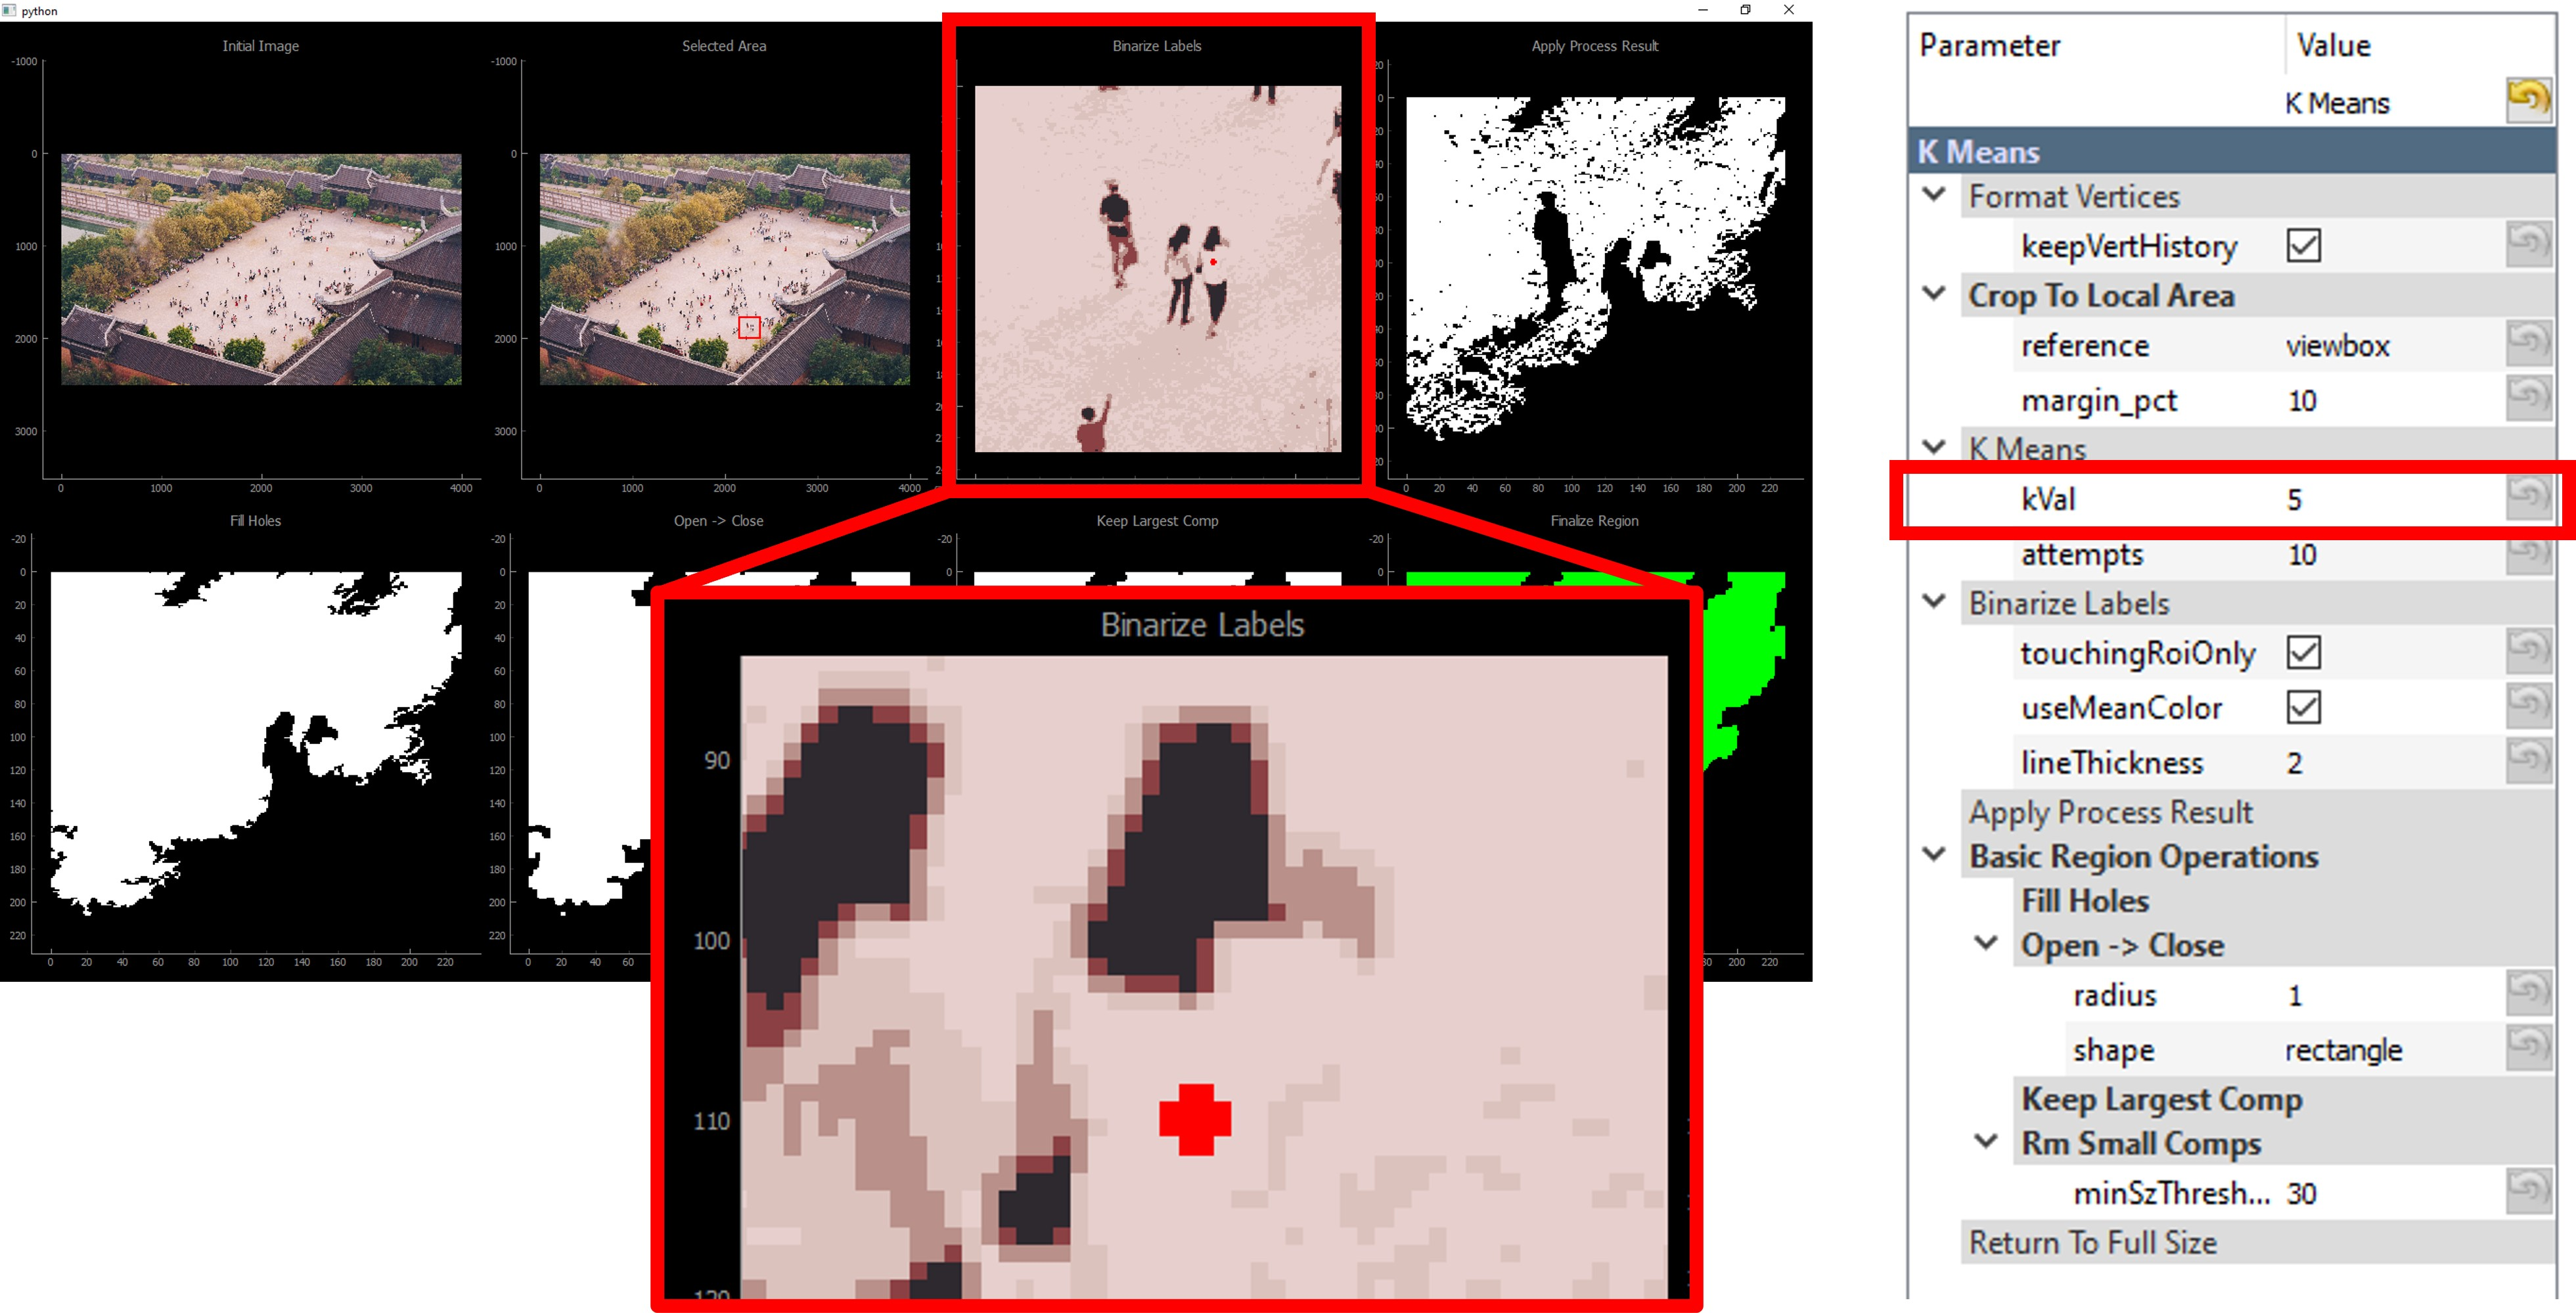
\includegraphics[width=0.7\linewidth]{figures/regionAnalytics}
    \caption{Outputs of each processing stage can be quickly viewed in context after an iteration of annotating. Upon inspecting the results, it is clear the failure point is a low $k$ value during K-means clustering and segmentation. The woman's shirt is not sufficiently distinguishable from the background palette to denote a separate entity. The red dot is an indicator of where the operator clicked during annotation.}
    \label{fig:regionAnalytics}
\end{figure*}
}

\newcommand{\makeRegionEditFig}{
\begin{figure}[tbp]
  \centering
  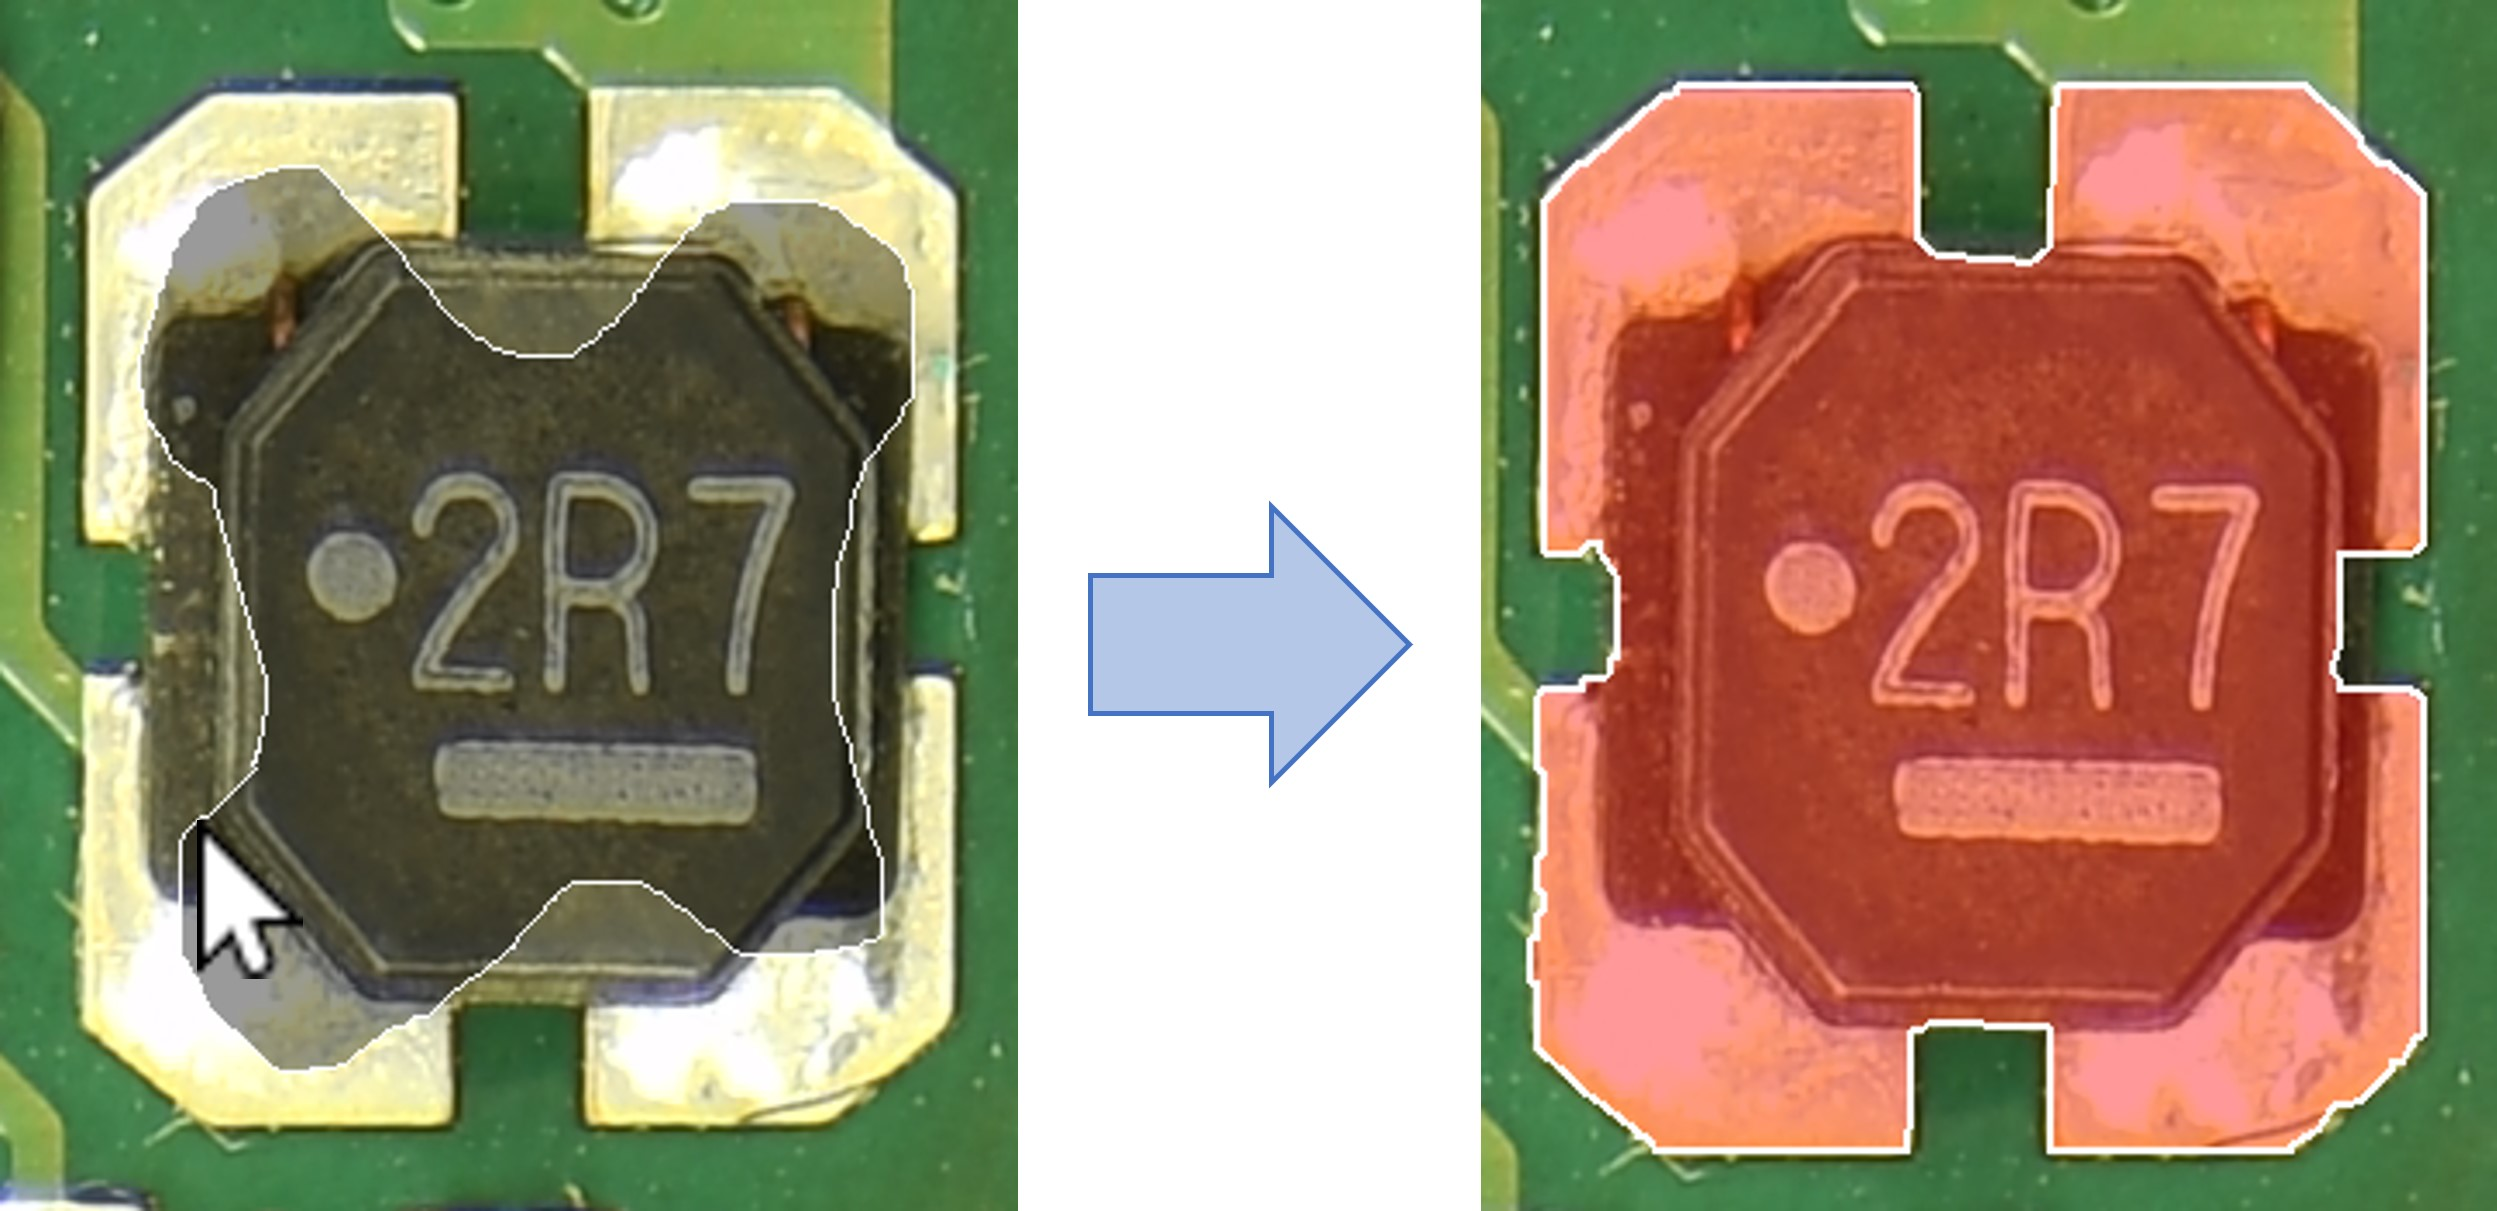
\includegraphics[width=\linewidth]{figures/regionEdit}
  \caption{Regardless of total image size and number of annotations, Python processing is be limited to the ROI or viewbox size for just the selected object based on user preferences. The depiction shows Grab Cut operating on a user-defined initial region within a much larger (8000x6000) image. The resulting region was available in 1.94 seconds on low-grade hardware.}
  \label{fig:regionEdit}
\end{figure}
}

\newcommand{\makeMetadataFig}{
\begin{figure}[tbp]
  \centering
  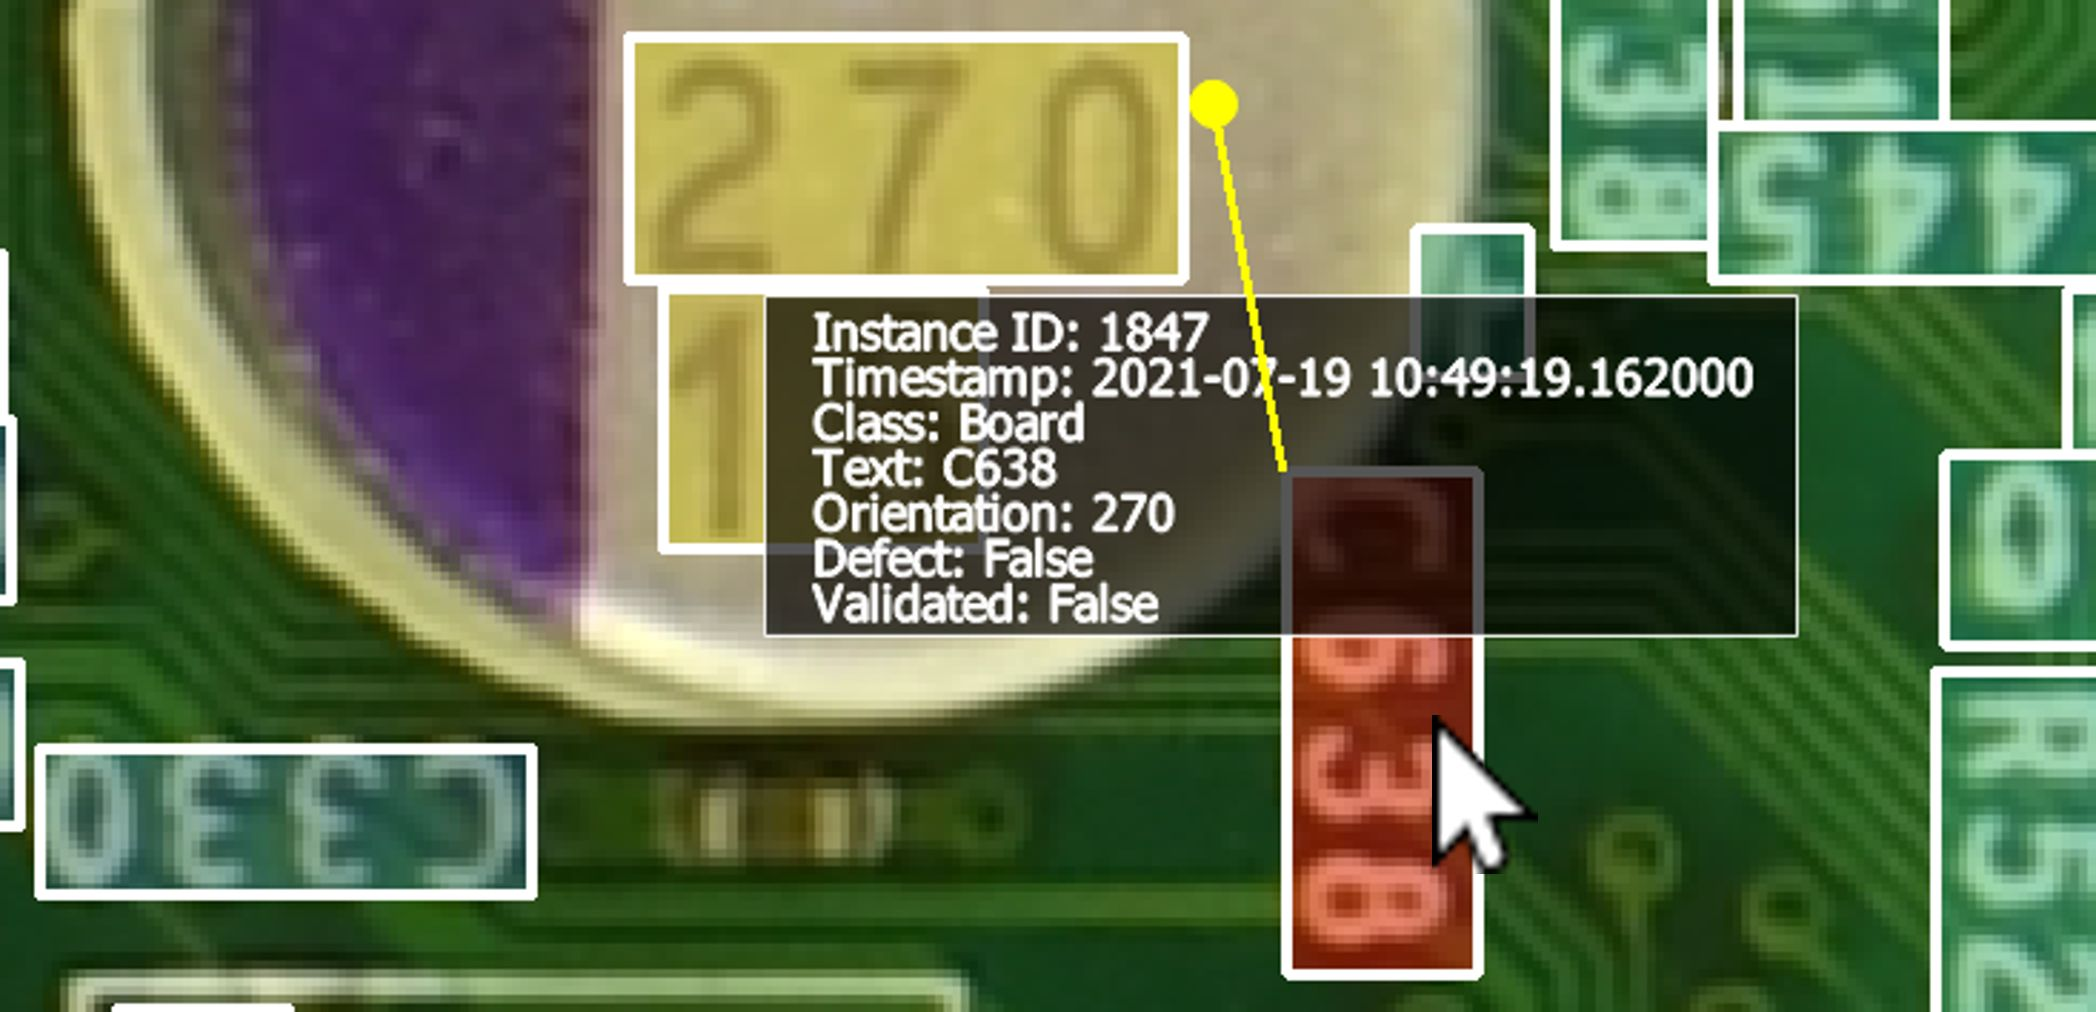
\includegraphics[width=\linewidth]{figures/metadata}
  \caption{Metadata can be collected, validated, and customized with ease. A mix of default properties (strings, numbers, booleans), factories (timestamp, author), and custom plugins (yellow circle representing associated device) are present.}
  \label{fig:metadata}
\end{figure}
}

\newcommand{\makeComplexRegionFig}{
\begin{figure}[tbp]
  \centering
  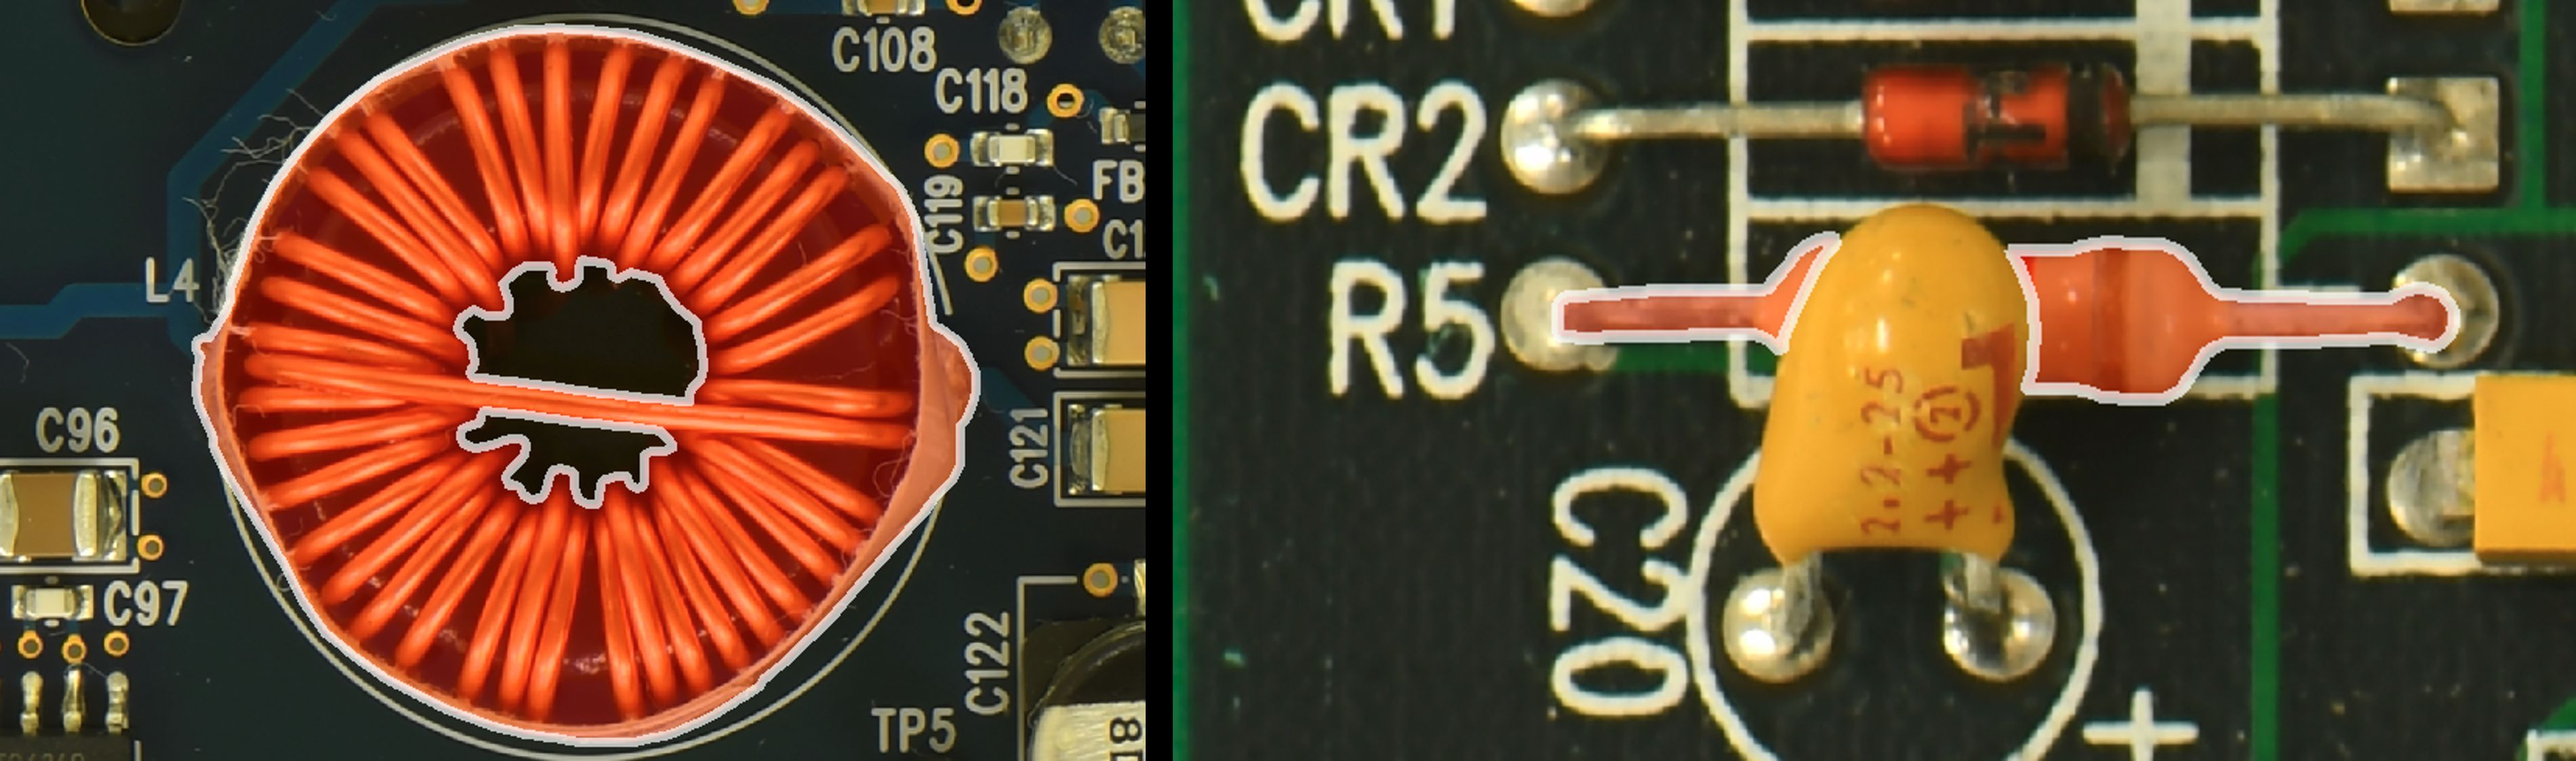
\includegraphics[width=\linewidth]{figures/complexRegion}
  \caption{Annotated objects in S3A can incorporate both holes and distinct regions through a multi-polygon container. Holes are represented as polygons drawn on top of existing foreground, and can be arbitrarily nested (i.e. island foreground is also possible).}
  \label{fig:complexRegion}
\end{figure}
}

% \newcommand{\makeSegComparisonFig}{%
% \begin{figure*}[hbtp]
% 	\centering
% 	\subfloat[Example PCB segmentation. In contrast to typical semgentation tasks, the scene contains over 4,000 objects with numerous complex shapes.]{%
% 		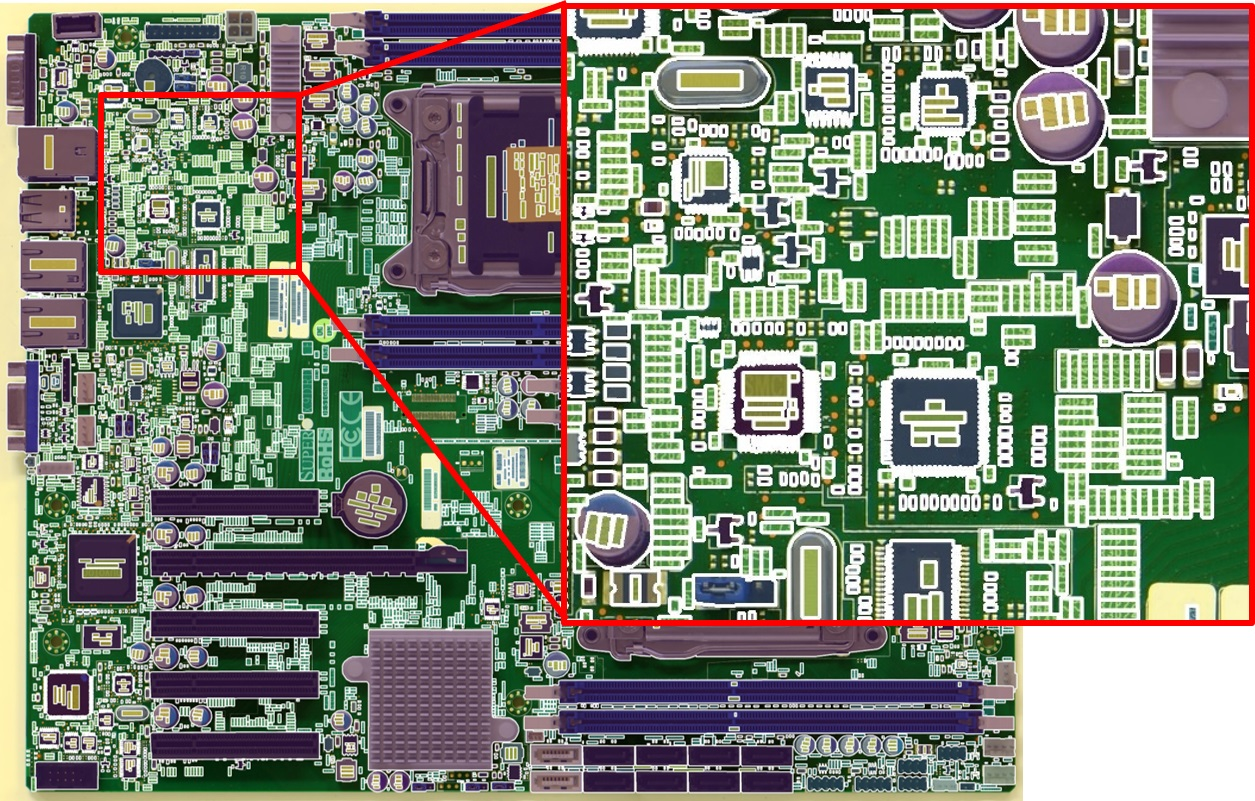
\includegraphics[width=0.6\linewidth]{figures/pcb}%
% 		\label{fig:pcb}
% 	}	
% 	\hfill
% 	\subfloat[Common use cases for semantic segmentation involve relatively few foreground objects, low-resolution data, and limited complexity per object. Images retrieved from \url{https://cocodataset.org/\#explore}.]{%
% 		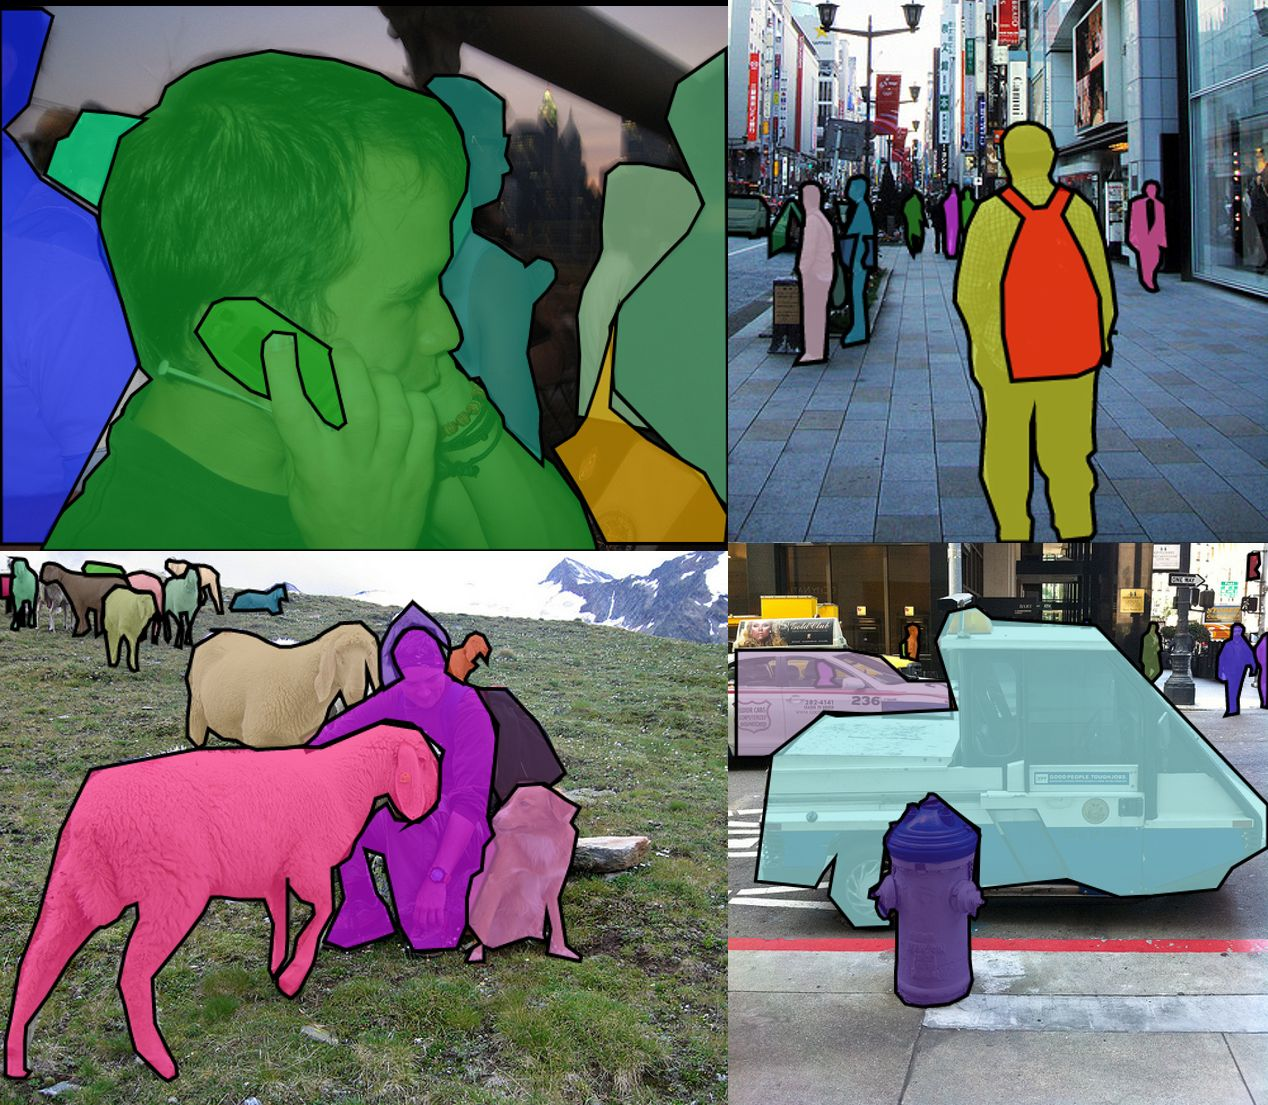
\includegraphics[width=0.42\linewidth]{figures/sampleSegData}%
% 		\label{fig:sampleSegData}
% 	}
% 	\caption{A comparison between a common PCB annotation versus COCO annotations reveals the significant differences between these datasets.}
% 	\label{fig:segComparison}
% \end{figure*}
% }

%% Paper title.
\title{Semi-Supervised Semantic Annotator (S3A): Toward Efficient Semantic Image Labeling}

%% This is how authors are specified in the journal style

%% indicate IEEE Member or Student Member in form indicated below
\author{Nathan Jessurun, Daniel E. Capecci, Olivia P. Dizon-Paradis, Damon L. Woodard, Navid Asadizanjani}
\begin{document}

\maketitle

\begin{abstract}
Most semantic image annotation platforms suffer severe bottlenecks when handling large images, complex regions of interest, or numerous distinct foreground regions in a single image. We have developed the Semi-Supervised Semantic Annotator (S3A) to address each of these issues and facilitate rapid collection of ground truth pixel-level labeled data. Such a feat is accomplished through a robust and easy-to-extend integration of arbitrary python image processing functions into the semantic labeling process. Importantly, the framework devised for this application allows easy visualization and machine learning prediction of arbitrary formats and amounts of per-component metadata. To our knowledge, the ease and flexibility offered are unique to S3A among all open-source alternatives. S3A is available through pypi.org (\url{https://pypi.org/project/s3a/}) and GitLab (\url{https://gitlab.com/s3a/s3a}).
\end{abstract}

\section{Introduction}
Labeled image data is essential for training, tuning, and evaluating the performance of many machine learning applications.
Such labels are typically defined with simple polygons, ellipses, and bounding boxes (i.e., ``this rectangle contains a cat").
However, this approach can misrepresent more complex shapes with holes or multiple regions as shown later in \autoref{fig:complexRegion}.
When high accuracy is required, labels must be specified at or close to the pixel-level - a process known as semantic labeling or semantic segmentation.
A detailed description of this process is given in \cite{chengSurveyAnalysisAutomatic2018}.
Examples can readily be found in several popular datasets such as COCO, depicted in \autoref{fig:sampleSegData}.

\makeSampleSegFig

Semantic segmentation is important in numerous domains including printed circuit board assembly (PCBA) inspection (discussed later in the case study) \cite{paradis2020color,azhaganReviewAutomaticBill2019}, quality control during manufacturing \cite{fergusonDetectionSegmentationManufacturing2018,anagnostopoulosComputerVisionApproach2001,anagnostopoulosHighPerformanceComputing2002}, manuscript restoration / digitization \cite{gatosSegmentationfreeRecognitionTechnique2004,kesimanNewSchemeText2016,jainTextSegmentationUsing1992,taxtSegmentationDocumentImages1989,fujisawaSegmentationMethodsCharacter1992}, and effective patient diagnosis \cite{seifertSemanticAnnotationMedical2010,rajchlDeepCutObjectSegmentation2017,yushkevichUserguided3DActive2006,iakovidisRatsnakeVersatileImage2014}.
In all these cases, imprecise annotations severely limit the development of automated solutions and can decrease the accuracy of standard trained segmentation models.

Quality semantic segmentation is difficult due to a reliance on large, high-quality datasets, which are often created by manually labeling each image.
Manual annotation is error-prone, costly, and greatly hinders scalability.
As such, several tools have been proposed to alleviate the burden of collecting these ground-truth labels~\cite{BestImageAnnotation}.
Unfortunately, existing tools are heavily biased toward lower-resolution images with few regions of interest (ROI), similar to \autoref{fig:sampleSegData}.
While this may not be an issue for some datasets, such assumptions are \emph{crippling} for high-fidelity images with hundreds of annotated ROIs~\cite{Ladicky_whatWhereCombiningCRFs,Wang_multiLabelImageAnnotation}.

With improving hardware capabilities and increasing need for high-resolution ground truth segmentation, there are a continually growing number of applications that \emph{require} high-resolution imaging with the previously described characteristics \cite{Mohajerani_cloudRemoteSensing,Demochkina_improvingOneShotXray}.
In these cases, the existing annotation tooling greatly impacts productivity due to the previously referenced assumptions and lack of support \cite{SpaceNet2020-lb}.

In response to these bottlenecks, \emph{we present the Semi-Supervised Semantic Annotation (S3A) annotation and prototyping platform -- an application which eases the process of pixel-level labeling in large, complex scenes.}\footnote{A preliminary version was introduced in an earlier publication~\cite{jessurunComponentDetectionEvaluation2020}, but significant changes to the framework and tool capabilities have been employed since then.}
Its graphical user interface is shown in \autoref{fig:appOverview}.
The software includes live app-level property customization, real-time algorithm modification and feedback, region prediction assistance, constrained component table editing based on allowed data types, various data export formats, and a highly adaptable set of plugin interfaces for domain-specific extensions to S3A.
Beyond software improvements, these features play significant roles in bridging the gap between human annotation efforts and scalable, automated segmentation methods \cite{Branson_humansInLoop}.

\makeAppOverviewFig

\section{Application Overview}\label{sec:appFeatures}
Design decisions throughout S3A's architecture have been driven by the following objectives: metadata should have significance rather than be treated as an afterthought; high-resolution images should have minimal impact on the annotation workflow; ROI density and complexity should not limit annotation workflow; and prototyping should not be hindered by application complexity.
These motives were selected upon noticing the general lack of solutions for related problems in previous literature and tooling.
Moreover, applications that \emph{do} address multiple aspects of complex region annotation often require an enterprise service and cannot be accessed under open-source policies.

While the first three points are highlighted in the case study, the subsections below outline pieces of S3A's architecture that prove useful for iterative algorithm prototyping and dataset generation as depicted in \autoref{fig:feedbackLoop}.
Note that beyond the facets illustrated here, S3A possesses multiple additional characteristics as outlined in its documentation (\url{https://gitlab.com/s3a/s3a/-/wikis/docs/User's-Guide}).

\makeFeedbackLoopFig

\subsection{Processing Framework}\label{sec:procFramework}
At the root of S3A's functionality and configurability lies its adaptive processing framework.
Functions exposed within S3A are thinly wrapped using a \texttt{Process} structure responsible for parsing signature information to provide documentation, parameter information, and more to the UI.
Hence, all graphical depictions are abstracted beyond the concern of the user while remaining trivial to specify (but can be modified or customized if desired).
As a result, incorporating additional/customized application functionality can require as little as one line of code.
Processes interface with PyQtGraph parameters to gain access to data-customized widget types and more (\url{https://github.com/pyqtgraph/pyqtgraph}).

These processes can also be arbitrarily nested and chained, which is critical for developing hierarchical image processing models, an example of which is shown in \autoref{fig:regionAnalytics}.
This framework is used for all image and region processing within S3A.
Note that for image processes, each portion of the hierarchy yields intermediate outputs to determine which stage of the process flow is responsible for various changes.
This, in turn, reduces the effort required to determine which parameters must be adjusted to achieve optimal performance.

\makeRegionAnalyticsFig

\subsection{Plugins for User Extensions}\label{sec:plugins}
The previous section briefly described how custom user functions are easily be wrapped within a process, exposing its parameters within S3A in a GUI format.
A rich plugin interface is built on top of this capability in which custom functions, table field predictors, default action hooks, and more can be directly integrated into S3A.
In all cases, only a few lines of code are required to achieve most integrations between user code and plugin interface specifications.
The core plugin infrastructure consists of a function/property registration mechanism and an interaction window that shows them in the UI.
As such, arbitrary user functions can be `registered` in one line of code to a plugin, where it will be effectively exposed to the user within S3A.

Plugin features are heavily oriented toward easing the process of automation both for general annotation needs and niche datasets.
In either case, incorporating existing library functions is converted into a trivial task directly resulting in lower annotation and higher labeling accuracy.

\subsection{Adaptable I/O}
An extendable I/O framework allows annotations to be used in a myriad of ways.
Out-of-the-box, S3A easily supports instance-level segmentation outputs, facilitating deep learning model training.
As an example, \autoref{fig:cropExports} illustrates how each instance in the image becomes its own pair of image and mask data.
When several instances overlap, each is uniquely distinguishable depending on the characteristic of their label field.
Particularly helpful for models with fixed input sizes, these exports can optionally be forced to have a uniform shape (e.g., 512x512 pixels) while maintaining their aspect ratio.
This is accomplished by incorporating additional scene pixels around each object until the appropriate size is obtained.
Models trained on these exports can be directly plugged back into S3A's processing framework, allowing them to generate new annotations or refine preliminary user efforts.
The described I/O framework is also heavily modularized such that custom dataset specifications can easily be incorporated.
In this manner, future versions of S3A will facilitate interoperability with popular formats such as COCO and Pascal VOC.

\makeCropExportsFig

\subsection{Deep, Portable Customizability}
Beyond the features previously outlined, S3A provides numerous avenues to configure shortcuts, color schemes, and algorithm workflows.
Several examples of each can be seen in the \href{https://gitlab.com/s3a/s3a/-/wikis/docs/user's-guide}{user guide}.
Most customizable components prototyped within S3A can also be easily ported to external workflows after development.
Hierarchical processes have states saved in YAML files describing all parameters, which can be reloaded to create user profiles.
Alternatively, these same files can describe ideal parameter combinations for functions outside S3A in the event they are utilized in a different framework.
\section{Case Study}\label{sec:casestudy}
Both the inspiration and developing efforts for S3A were initially driven by optical printed circuit board (PCB) assurance needs.
In this domain, high-resolution images can contain thousands of complex objects in a scene, as seen in \autoref{fig:pcb}.
Moreover, numerous components are not representable by cardinal shapes such as rectangles, circles, etc.
Hence, high-count polygonal regions dominated a significant portion of the annotated regions.
The computational overhead from displaying large images and substantial numbers of complex regions either crashed most annotation platforms or prevented real-time interaction.
In response, S3A was designed to fill the gap in open-source annotation platforms that addressed each issue while requiring minimal setup and allowing easy prototyping of arbitrary image processing tasks.
The subsections below describe how the S3A labeling platform was utilized to collect a large database of PCB annotations along with their associated metadata\footnote{For those curious, the dataset and associated paper are accessible at \url{https://www.trust-hub.org/\#/data/pcb-images}.}.

\makePcbFig

\subsection{Large Images with Many Annotations}
In optical PCB assurance, one method of identifying component defects is to localize and characterize all objects in the image.
Each component can then be cross-referenced against genuine properties such as length/width, associated text, allowed orientations, etc.
However, PCB surfaces can contain hundreds to thousands of components at several magnitudes of size, necessitating high-resolution images for in-line scanning.
To handle this problem more generally, S3A separates the editing and viewing experiences.
In other words, annotation time is orders of magnitude faster since only edits in one region at a time and on a small subset of the full image are considered during assisted segmentation.
All other annotations are read-only until selected for alteration.
For instance, \autoref{fig:regionEdit} depicts user inputs on a small ROI out of a much larger image.
The resulting component shape is proposed within seconds and can either be accepted or modified further by the user.
While PCB annotations initially inspired this approach, it is worth noting that the architectural approach applies to arbitrary domains of image segmentation.

Another key performance improvement comes from resizing the processed region to a user-defined maximum size.
For instance, if an ROI is specified across a large portion of the image but the maximum processing size is 500x500 pixels, the processed area will be downsampled to a maximum dimension length of 500 before intensive algorithms are run.
The final output will be upsampled back to the initial region size.
In this manner, optionally sacrificing a small amount of output accuracy can drastically accelerate runtime performance for larger annotated objects.

\makeRegionEditFig

\subsection{Complex Vertices/Semantic Segmentation}
Multiple types of PCB components possess complex shapes which might contain holes or noncontiguous regions.
Subsequently, it is beneficial for software like S3A to represent these features inherently with a \texttt{ComplexXYVertices} object: that is, a collection of polygons which either describe foreground regions or holes.
Subsequently, any possible shape or shape grouping can be represented as needed.
Example components difficult to accomodate with single-polygon annotation formats are illustrated in \autoref{fig:complexRegion}.

\makeComplexRegionFig

At the same time, S3A also supports high-count polygons with no performance losses.
Since region edits are performed by image processing algorithms, there is no need for each vertex to be manually placed or altered by human input.
Thus, such non-interactive shapes can simply be rendered as a filled path without a large number of event listeners present.
This is the key performance improvement when thousands of regions (each with thousands of points) are in the same field of view.
When low polygon counts \emph{are} required, S3A also supports RDP polygon simplification down to a user-specified epsilon parameter~\cite{ramer_iterative_1972}.

\subsection{Complex Metadata}
Most annotation software support robust implementation of image region, class, and various text tags (``metadata").
However, this paradigm makes collecting type-checked or input-sanitized metadata more difficult.
This includes label categories such as object rotation, multiclass specifications, dropdown selections, and more.
In contrast, S3A treats each metadata field the same way as object vertices, where they can be algorithm-assisted, directly input by the user, or part of a machine learning prediction framework.
Note that simple properties such as text strings or numbers can be directly input in the table cells with minimal need for annotation assistance\footnote{For a list of input validators and supported primitive types, refer to PyQtGraph's \href{https://pyqtgraph.readthedocs.io/en/latest/parametertree/parametertypes.html}{Parameter} documentation.}.
In conrast, custom fields can provide plugin specifications which allow more advanced user interaction.
Finally, auto-populated fields like annotation timestamp or author can easily be constructed by providing a factory function instead of default value in the parameter specification.

This capability is particularly relevant in the field of optical PCB assurance.
White markings on the PCB surface, known as silkscreen, indicate important aspects of nearby components.
Thus, understanding the silkscreen's orientation, alphanumeric characters, associated component, logos present, and more provide several methods by which to characterize / identify features of their respective devices.
Both default and customized input validators were applied to each field using parameter specifications, custom plugins, or simple factories as described above.
A summary of the metadata collected for one component is shown in \autoref{fig:metadata}.

\makeMetadataFig

\section{Conclusion and Future Work}
The Semi-Supervised Semantic Annotator (S3A) is proposed to address the difficult task of pixel-level annotations of image data.
For high-resolution images with numerous complex regions of interest, existing labeling software faces performance bottlenecks attempting to extract ground-truth information.
Moreover, there is a lack of capabilities to convert such a labeling workflow into an automated procedure with feedback at every step.
Each of these challenges is overcome by various features within S3A specifically designed for such tasks.
As a result, S3A provides not only tremendous time savings during ground truth annotation, but also allows an annotation pipeline to be directly converted into a prediction scheme.
Furthermore, the rapid feedback accessible at every stage of annotation expedites prototyping of novel solutions to imaging domains in which few examples of prior work exist.
Nonetheless, multiple avenues exist for improving S3A's capabilities in each of these areas.
Several prominent future goals are highlighted in the following sections.

\subsection{Dynamic Algorithm Builder}
Presently, processing workflows can be specified in a sequential YAML file which describes each algorithm and their respective parameters.
However, this is not easy to adapt within S3A, especially by inexperienced annotators.
Future iterations of S3A will incoroprate graphical flowcharts which make this process drastically more intuitive and provide faster feedback.
Frameworks like Orange~\cite{demsar_orange_2013} perform this task well, and S3A would strongly benefit from adding the relevant capabilities.

\subsection{Image Navigation Assistance}
Several aspects of image navigation can be incorporated to simplify the handling of large images.
For instance, a ``minimap" tool would allow users to maintain a global image perspective while making local edits.
Furthermore, this sense of scale aids intuition of how many regions of similar component density, color, etc.
exist within the entire image.

Second, multiple strategies for annotating large images leverage a windowing approach, where they will divide the total image into several smaller pieces in a gridlike fashion.
While this has its disadvantages, it is fast, easy to automate, and produces reasonable results depending on the initial image complexity \cite{Vigueras_fullCnnCornealSegmentation}.
Hence, these methods would be significantly easier to incorporate into S3A if a generalized windowing framework was incorporated which allows users to specify all necessary parameters such as window overlap, size, sampling frequency, etc.
A preliminary version of this is implemented for categorical-based model prediction, but a more robust feature set for interactive segmentation is strongly preferable.

\subsection{Aggregation of Human Annotation Habits}
Several times, it has been noted that manual segmentation of image data is not a feasible or scalable approach for remotely large datasets.
However, there are multiple cases in which human intuition can greatly outperform even complex neural networks, depending on the specific segmentation challenge \cite{Russakovsky_humanCollabAnnotation2015}.
For this reason, it would be ideal to capture data points possessing information about the human decision-making process and apply them to images at scale.
This may include taking into account human labeling time per class, hesitation between clicks, relationship between shape boundary complexity and instance quantity, and more.
By aggregating such statistics, a pattern may arise which can be leveraged as an additional automated annotation technique.


\printbibliography
\end{document}

